\chapter{Theoretical Foundation}
\label{chap:theory}

The following chapter provides a theoretical foundation for the research conducted in this thesis. It introduces the basic concepts of material flow planning and simulation, digital twins, process mining, and verification, validation, and uncertainty quantification (VVUQ). The relevance of these concepts in the context of simulation-based digital twins and their application in corporate practice will also be discussed.


\section{Discrete Material Flow Systems and Simulation}
This section begins with an introduction of the underlying concepts of Discrete Material Flow Systems (DMFS) and Simulation Based Digital Twins (SBDT).
\label{sec:material-flow}
\subsection{Basic Concepts}
Discrete material flow systems cannot be fully understood without first clarifying the principles of Discrete Event Simulation (DES) for Discrete Event Systems. In DES, a system changes its state through \textit{events} that occur at specific, discrete time instances; it is assumed that no changes occur between two successive events. Consequently, the state of the system is completely defined by the values of its descriptive variables at each event occurrence \autocite{varga2001discrete}. The time at which an event occurs is typically marked by a timestamp, and the scientific observation of such systems is conducted by analyzing the discrete \textit{sequence} of events over time \autocite{robinson2014simulation}.

Simulation, in this context, refers to the process of imitating the operation of a Discrete Event System over time—often through multiple event sequences. This imitation is captured in a model, and the core activities in a simulation involve constructing and experimenting with this model. A high-quality simulation abstracts the essential features of the system, which requires the modeller to have a sound a priori understanding of what “essential” means in the given context. Although the model can later be refined, its quality is primarily measured by its ability to predict outcomes and offer a diverse range of scenarios \autocite{maria1997introduction}.

In the context of DMFS, their simulation describes the imitation of material flow systems by breaking down continuous flows into discrete events. Such material flow systems can be characterized as “systems processing discrete objects (parts) that move at regular or irregular intervals along transportation routes or conveyor lines, comprising production and logistic systems” \autocite{Arnold2006,schwede2024learning}. These systems form the backbone of material flow planning and control structures. The central idea of material flow planning and control is to ensure that material requirements—both in terms of quantity and timing—are met during transportation and storage across the various stages of the supply chain \autocite{Gehr2007}. Importantly, the time horizon of interest spans from order placement up to delivery.
To summarize, DMFS are often simulated using DES, which abstracts the continuous flow of materials into discrete events. The simulation is carried out using a model. The simulation and modeller are embedded in the context of material flow planning and control, which aims to ensure that material requirements are met across the supply chain. Successfully performed material flow planning and control induce high quality data for simulation and modelling purposes.

\subsection{Comparing DMFS}
\label{sec:comparing-dmfs}
Because the simulation of DMFS often involves (discrete) event simulation, events in DMFS need to be further differentiated to be comparable. \Autocite{Arnold2006} propose to differentiate DMFS into static and dynamic components.

Static components describe the possible states of the system. Possible states can be the set of possible processes given a part or resource, for example. Dynamic components define the concrete material flow for a certain part or order.
Static components include parts, resources and processes \autocite{schwede2024learning}. Parts are transformed by processes using resources sometimes based on orders. Transformation can have an impact on physical properties of the parts (transformation model), spatial position (transition model), the quality of the parts (quality model) and takes time (time model) and uses resources (resource model). Resources have a capacity of handling parts in parallel (resource capacity model) and processes have a predecessor-successors relationship (process model).
Dynamic components are used to define the concrete dynamic material flow within the DMFS. There are four components: Order generation, order control, resource control and supply control. Order generation defines the load the system must process. Order control defines how parts are processed, sometimes referred to as routing rules \autocite{mildeautomated}. Resource control defines how resources decide to handle processing requests, also sometimes referred to as priority rules. Supply control describes how supply parts are provided \autocite{mildeautomated,schwede2024learning}. See the latter source for a more detailed description of the components.


\subsection{Production Planning and Control}
\label{sec:ppc}
Successful companies use production planning and control frameworks to describe and optimize their DMFS. After establishing a theoretical foundation and simulation approaches for DMFS, this section thus focusses on Production Planning and Control (PPC) as a critical factor influencing the quality and quantity of data generated by Discrete Event Simulation.
PPC is the structured approach to planning, scheduling, controlling and managing all aspects of the manufacturing process. It involves the coordination of resources, processes, and orders to meet production goals. PPC is essential for optimizing production processes, reducing costs, and improving quality. The main functions of PPC include production planning, production scheduling, and production control. Production planning involves determining the production capacity, production goals, and production processes. Production scheduling involves creating a detailed schedule for production activities. Production control involves monitoring and controlling production activities to ensure that production goals are met \autocite{kiran2019production}. Scheduling is usually the last step performed before execution of the plan \autocite{pinedo2012design}.

The integration of PPC with simulation models is crucial because it directly affects the data quality used in DES of DMFS. Effective PPC processes anticipate anomalies in the production cycle, allowing for adjustments that maintain system efficiency and reliability. If successful, these adjustments yield high-quality data that enhance the accuracy of simulation outcomes. \autocite{kiran2019production}.


\subsection{Relevant KPIs and Metrics}
\label{sec:relevant-kpis}
Up to this point, DES for SBDT of DMFS has been introduced, outlining the key factors that contribute to a robust simulation. A model differentiation framework proposed by \citeauthor*{schwede2024learning} has been briefly presented to facilitate comparison of SBDT. Furthermore, the critical role of PPC in generating high-quality data for simulation has been discussed. These discussions ignored up till now that, even when SBDT are integrated within well-functioning PPC processes, various SBDT models remain prone to errors and inherent trade-offs that must be addressed by the modeller \autocite{Tao2018ijamt}.

The goal conflict of the modeller when developing SBDT can be described by the following conflict triangle \autocite{robinson2014simulation,balci2012life}:

\begin{figure}[htbp]
  \centering
  
\includegraphics[width=0.8\textwidth]{figures/goals.png}
  \caption{The goal conflict of the modeller when developing SBDT. Aiming for higher accuracy (validity) often leads to higher computational costs (efficiency) and reduced scalability (applicability). Reaching more efficiency often leads to reduced accuracy and scalability. Aiming for higher scalability often leads to reduced accuracy and efficiency.}
  \label{fig:goals}
\end{figure}

Focusing one of the three dimensions—accuracy (validity), efficiency (computation time), and applicability (scalability)—often leads to trade-offs in the other two dimensions. Oftentimes the data itself is not sufficient to make a decision on which trade-off to make. Limited data points may hinder the modeller from reaching high validity. System architecture may block the system from reaching good scalability. Hardware limitations may hinder the modeller from reaching high efficiency.
At other times, corporate management may have a preference for one of the dimensions.

One solution to balance and quantify these goals can be achieved by defining a set of KPIs. Some may already be available through PPC, some may be calculated from DES data or the DES itself. Optimally, the data warehouse provides relevant views \autocite{cui2020manufacturing}. Because the SBDT in theory mirrors the DMFS, the KPIs gathered from PPC and the DES should yield identical values. Deviations between the KPIs of the SBDT and the DMFS may indicate errors in the SBDT or anomalies in the DFMS. The following KPIs are relevant for the evaluation of SBDT:

\begin{figure}[htbp]
  \centering
  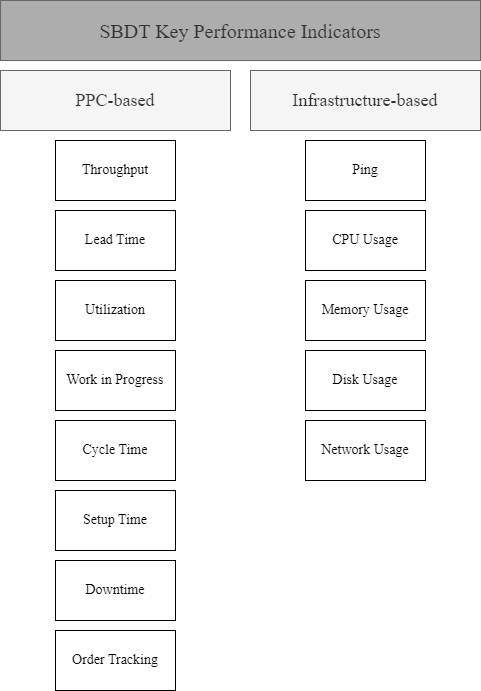
\includegraphics[width=0.8\textwidth]{figures/kpi.png}
  \caption{SBDT KPIs differentiated by PPC-based and Infrastructure-based indicators.}
  \label{fig:kpis}
\end{figure}

The PPC related KPIs may be provided by above mentioned data warehouse, because they are highly relevant in the context of production scheduling and -control. Throughput measures the number of produced parts at the last station in a specified period. It is an indicator for the productivity of the manufacturing sytem \autocite{imseitif2019throughput}. Lead time is the cumulative time a part travels through the system from start to sink. It is an indicator for the efficiency of the manufacturing system \autocite{pfeiffer2016manufacturing}. Cycle time measures the same amount like lead time but focusses only on the active production process, excluding transports and waiting times \autocite{griffin1993metrics}. Setup time measures the time needed to prepare a machine for a new task. It is an indicator for the flexibility of the manufacturing system \autocite{allahverdi2008significance}. In the given usecase, we aggregate the setup time for all setup processes. All KPIs presented so far can be calculated dynamically when new data has been sent. Later on, they may serve as an alert system for the modeller to detect deviations between the SBDT and the DMFS, see \autoref{sec:vvuq-sbdt}.

The infrastructure related KPIs are derived by sensors from the executing system of the SBDT. Ping time measures the time needed to send a signal from one point to another. It is an indicator for the latency of the infrastructure \autocite{wu2021digital}. SBDT need to enforce real-time control over the physical entity. The latency thus needs to be as low as possible. In this scenario, one point (sender) is represented by the physical entity and its sensors. The receiving point runs the SBDT. It is advantageous to run the SBDT on Edge to minmize latency- and transmission costs \autocite{li2018learning}. CPU-, memory-, disk- and network usage metrics are indicators for the load of the infrastructure. They are important to detect bottlenecks in the infrastructure \autocite{li2018learning}. The first indicator is usually measured in percent of the maximum CPU capacity. The latter three indicators are usually measured in bytes or bits per second \autocite{granelli2021evaluating}.


\section{Digital Twin: Definition and Concepts}
\label{sec:digital-twin}
The latter section gave a short intrduction into DFMS, DES, its metrics and the corporate processes accompanying the SBDT. Now, we shed light on the DT itself. For a short introduction to the topic, see \autoref{chap:introduction}.

Like introduced in the predecessing chapter, DT inherent the highest order of modelling fidelity compared to DM or DS. There are different definitions of DT present in the literature \autocite{Negri2017promfg,zheng2019application,glaessgen2012digital,Demkovich2018def,boschert2016digital,grieves2014digital,kritzinger2018digital,Tao2018ijamt,zehnder2018representing}. Each of them highlights different aspects of the DT. This thesis uliziles the definition by \autocite{grieves2014digital} which highlights the conceptual elements of the twin and its lifecylce focus:

\begin{quote}
  The digital twin concept (...) contains three main parts: A) Physical products in real space, (B) virtual products in virtual space and (C) the two-way connections of data and information that tie the virtual and real products together. \autocite{grieves2014digital}
\end{quote}

The physical product is the entity which will be modelled. The virtual product is the DT itself, but also its infrastructure, for example data services making the real-time data flow possible \autocite{Tao2018ijamt}. The two-way connection is the data flow between the physical and the virtual product. The data flow is bidirectional. \citeauthor{zehnder2018representing} add that the data flow may contain meta data "describing the data source and its context". Also the connection protocol is of importance here (e.g. MQTT or REST). TCP may be the method of choice as it ensures that the packages arrive in the correct order and without errors \autocite{li2018learning}.

\subsection{Types of Digital Twins}
\label{sec:types-digital-twins}
Now that a unified understanding of DT has been established, this section focuses on how DT may be learned from different sources of information. The following list includes the most relevant types of DT with a focus on different kinds of information sources:

\begin{itemize}
  \item Simulation-based DT (SBDT) \autocite{Lugaresi2021aifac,martinez2018automatic}
  \item Data-driven DT (DDDT) \autocite{he2019data,Friederich2022}
  \item Hybrid Digital Twins (HDT) \autocite{luo2020hybrid,huang2023hybrid}
\end{itemize}


SBDTs \autocite{Lugaresi2021aifac,martinez2018automatic,boschert2016digital} are based on DES. They utilize discrete event simulation (see \autoref{sec:material-flow}) to create a dynamic representation of the physical system \autocite{schluse2016simulation,pantelides2013online}. To incorporate a SBDT into workflows and processes, suitable data structures must be in place beforehand \autocite{boschert2016digital}. DES may improve the predictive capabilities of the model compared to manual twin creation. DES is able to model causal relationships between the events \autocite{francis2021towards}. In contrast, the development of a realistic simulation model requires experts and time \autocite{Charpentier2014}. If the simulation model fails to capture recent behaviour of the physical entity, a recalibration is mandatory \autocite{Friederich2022}. To conclude, SBDTs are a step forward to speed up the creation and updating processes of DTs.

DDDT rely on the utilization of data to model the physical entity. The data may be gathered from sensors, data warehouses or other sources. The data is used to train a model which represents the physical entity. The model may be a neural network, a decision tree or another machine learning model. The model is then used to predict future states of the physical entity. The model may be updated with new data to increase its accuracy \autocite{he2019data,Friederich2022}. For a more detailed description of DDDT including its up- and downsides, see \autoref{sec:data-driven-digital-twins}.

HDT combine different sources of information to create a more accurate model of the physical entity. The sources may be simulation models (see \autoref{sec:material-flow}), data-driven models (see \autoref{sec:data-driven-digital-twins}) or physics-based models. Physics-based models contain information about the physical properties and behaviors of the entity. They do not have to learn these characteristics from the data because this information is made available to the model \textit{a priori} \autocite{kapteyn2022data,aivaliotis2019methodology}. The simulation based models accompanying the physics-based one obeys characteristics of SBDT, see above. The combination of different sources may make the HDT more robust and a faster learner. HDT unite the advantages of SBDT with the knowledge advantage physics based models have. Unfortunately, they also inherit the disadvatages of SBDT. Physics-based models may also involve heavy involve heavy computational costs and domain expertise \autocite{kapteyn2022data}.

\subsection{Data-Driven Digital Twins}
\label{sec:data-driven-digital-twins}

While SBDTs and HDT possess not negligible computational costs and require domain expertise, DDDT are able to learn from data without the need for a hand-written simulation model. The DDDT \textit{learns} the model. Learning in the context of DDDT is not trivial, several approaches have been proposed in the literature \autocite{he2019data,Friederich2022,francis2021towards}. Often times Data Science methods come to work. The learning process may be supervised or unsupervised. Supervised learning uses labeled data to train the model \autocite{cunningham2008supervised}. The label can symbolize different values of interest. Unsupervised learning uses unlabeled data to train the model \autocite{barlow1989unsupervised}. Often times, the task at hand is to group the data into different categories. Data sources of interest may be process data, resource data or order data \autocite{Biesinger2019}.
The learning process may be online or offline. Offline learning uses the data \textit{once} for training, validation and testing, while online learning continuously updates the model with new data to adapt to changes in the physical system. Online learning is thus able to capture new trends in the data and to foresee concept drift \autocite{tsymbal2004problem}. DDDT have to be differentiated from data-driven simulation \autocite{Charpentier2014}, which involves human invervention to create highly individual solutions for the physical entity. The key difference is that every characteristic has to be explicitly described in the model by the expert, there are no efforts to let an intelligent algorithm learn these by itself. DDDT may be able to update themselves to new trends in the data by online learning, termed \textit{syncronization} \autocite{reinhardt2019survey}. Latter has to be differentiated from \textit{updating}, which is a manual process to take corrective action in the logic of the twin itself \autocite{schwede2024learning}. An example for updating a DDDT may be the addition of a new feature to the model. An example for synchronization may be the adaption of the model to new trends in the data. The latter may be done by the model itself, the former has to be done by the modeller.
DDDT thus rely less on domain expertise and manual model creation. A suitable model may be able to capture relevant trends in the data and to predict outcomes which describe most of the characteristics of the physical entity. \autocite{francis2021towards} propose several key elements a DDDT must contain to be termed \textit{data-driven}:

\begin{enumerate}
  \item \textbf{Data Collection:} The relevant entities to be modelled have to be identified. This activity involves data gathering of the identified entities and ensuring a steady data stream to a database. The data may be gathered from sensors, data warehouses or other sources.
  \item \textbf{Data Validation:} This step involves cleaning and preprocessing the data. The data may contain missing values, outliers or other errors. The data has to be cleaned and preprocessed to ensure a high quality of the model. Plausibility checks may be performed to ensure the data is correct.
  \item \textbf{Knowledge Extraction:} After the data has been collected and cleaned, events have to be detected. \Citeauthor{francis2021towards} utilize process mining terms in this context, such as evemt detection and process discovery. The main goal in this step is to find a common ground on which events are of interest. The thesis later dives deeper into Process Mining techniques applied here, see \autoref{sec:process-mining}.
  \item \textbf{(Semi-)automatic Simulation Modeling:} The data is used to train a model. This step may use offline or online data as a stream. The model may be a neural network, a decision tree or another machine learning model. The model is then used to predict future states of the physical entity. The model may be updated with new data to increase its accuracy.
  \item \textbf{Continuous Model Validation:} Interestingly,\citeauthor{francis2021towards} propose a continuous model validation. In the online learning case, they recommend to use the steady data stream to apply validation techniques continuously, see \autoref{sec:vvuq-sbdt} The validation may be performed by comparing the model predictions with the real data. If the model deviates from the real data, the model may be recalibrated.
\end{enumerate}

DDDTs go one step further than SBDT and minimize the influence of the human in the loop \autocite{francis2021towards,Friederich2022}. Faster model development and updating activities are the result. The third reason to automate DT endevours elaborated by \citeauthor{schwede2024learning}, increasing prediction quality, rises and falls with the data quality, thus the gathering and preprocessing efforts of the modeller. Extrinsic factors like the number of data points available also play into the equation. If the number of features is greater than the number of samples, the curse of dimensionality hinders a good modelling performance \autocite{koppen2000curse}. DDDT should avoid biased or noisy predictions at all costs. The identification of \textit{relevant} events poses the risk of introducing a selection bias, rather a confirmation bias. The modeller may have the tendency to select events which confirm his or her hypothesis. Ramdom sampling may be a solution to this problem, but can destroy sequential information patterns in event sequences. Overall DDDT are a promising approach to model the physical entity. If the right balance between human involvement and automated learning is found, it may be an efficient solution \autocite{francis2021towards}. Thinking one step ahead, employing data-based VVUQ approaches may also be a gamechanger. This topic will be discussed in Section \autoref{sec:ml_validation}.

\label{par:asmg}
One last discipline, automatic simulation model generation (ASMG), is worth mentioning. ASMG has to be differentiated from DDDT by the effort to automatically generate models, thus DM and DS through DES. Automatic DT generation is not necessarily the goal. It aims to automate the model generation process and tries to eliminate the human in the loop, \autocite{reinhardt2019survey,lechevalier2018methodology}. Automation is achieved by taking into account a diverse range of data sources, including Computer Aided Design data, PPS data, production manuals, process data and programming code, thus reaching a high data variability. The gathered data has to be processed online or offline as well through suitable frameworks or human intervention. Challenges lay in incomplete data \autocite{bergmann2014automatische}, although the same problems of DDDT also apply here. If the gained data is not mined thoroughly, human intervention is needed again, mitigating automation efforts.

To conclude this section about DT, the thesis summarizes that there are different types of DT differentiated by their source of information retrieval. A lot of work has been done to make the DT creation, updating and prediction process more efficient. By the help of simulation, data and automated model generation, the DT may be created with less time and resources than manually.

\section{Process Mining and Event Logs}
\label{sec:process-mining}
After we introduced the corporate embedding of DTs and their types, the thesis now focusses on process mining (PM) and event logs. PM is a discipline which aims to extract knowledge from event logs. Event logs are the data basis for PM. The following section introduces the basic concepts of PM and event logs.

\subsection{Core Concepts}
\label{sec:core-concepts}
PM is a discipline established 1999 which is interdisciplinary rooted in the field of Data Science and Process Science \autocite{van2016data}. Data Science can be considered a process agnostic discipline \autocite{van2016data} while process science uses models not covering hidden trends in the data. The bridge between both approaches is PM. The goal of PM is to use event data to identify and extract process information \autocite{vanderAalst2012}. This information is used to discover (process discovery), monitor (conformance checking) and improve processes (process enhancement) \autocite{vanderAalst2012} by using event logs. Such logs must contain a case ID, an activity name and a timestamp. Additional information like resource informations, order informations or other context information may be added to the log \autocite{vanderAalst2012}. Such logs assume that the process can be captured fully and sequentially.

\begin{table}[htbp]
  \centering
  \caption{A fragment of a manufacturing event log: Each line corresponds to an event. The case ID groups unique events which are identified by an event ID to one group, a trace. The timestamp refers to the time of event occurrence, while the activity describes the event. In this example, additional information like resource name and cost are given as well. Case 1, for example, consists of five events, involving a warehouse, two inspectors, and one machine.}
  \label{tab:manufacturinglog}
  \resizebox{\textwidth}{!}{%
    \begin{tabular}{r r l l l r}
      \toprule
      \textbf{Case id} & \textbf{Event id} & \textbf{Timestamp} & \textbf{Activity}     & \textbf{Resource} & \textbf{Cost} \\
      \midrule
      1                & 101               & 10-01-2025:08.00   & receive raw material  & Warehouse A       & 500           \\
                       & 102               & 10-01-2025:08.30   & initial quality check & Inspector Bob     & 300           \\
                       & 103               & 10-01-2025:09.00   & cutting process       & Machine X         & 800           \\
                       & 104               & 10-01-2025:09.45   & assembly              & Worker Alice      & 600           \\
                       & 105               & 10-01-2025:10.30   & final inspection      & Inspector Eve     & 400           \\
      \midrule
      2                & 201               & 11-01-2025:07.45   & receive raw material  & Warehouse B       & 500           \\
                       & 202               & 11-01-2025:08.15   & cutting process       & Machine Y         & 800           \\
                       & 203               & 11-01-2025:09.00   & welding               & Robot Arm Z       & 700           \\
                       & 204               & 11-01-2025:09.45   & quality assurance     & Inspector Dave    & 400           \\
      \midrule
      3                & 301               & 12-01-2025:06.30   & receive raw material  & Warehouse C       & 500           \\
                       & 302               & 12-01-2025:07.00   & initial quality check & Inspector Judy    & 300           \\
                       & 303               & 12-01-2025:07.30   & CNC machining         & Machine W         & 900           \\
                       & 304               & 12-01-2025:08.15   & painting              & Worker Karl       & 500           \\
                       & 305               & 12-01-2025:09.00   & packaging             & Worker Laura      & 350           \\
      \bottomrule
    \end{tabular}%
  }
\end{table}

\autoref{tab:manufacturinglog} illustrates the PM concepts. The case ID groups unique events which are identified by an event ID to one group, a trace. The timestamp refers to the time of event occurence, while the activity describes the event. In this example, additional informations like resource name and cost are given as well. Cases containing the same events identified by unique event IDs will have different case IDs \autocite{van2016data}. Process discovery may try to produce a process model from the event log. The model may be a Petri net, a BPMN model or another process model. The challenge lies not in the recording of every trace present in the event log, rather in finding a generic representation of the most occuring traces. The process model must be generic enough to describe most traces, but specific enough to not get invalidated by future traces which may contain completely different events. Another major building block of this process model is accounting for trace concurrency. When several events may be identified to happen in parallel during the same time window, the model must recognize this. It can be spoken of a classical bias-variance tradeoff lend from data science. The process most contain the most frequent traces but has to filter out traces which contain anomalies. Such anomalies like longer time per event due to a fire alarm have to be accounted for. Conformance checking may compare a given process model against a given event log. They are specialized in detecting aforementioned anomalies. A key insight in conformance checking lies in two possible deviations from reality: The given model does not capture the real behaviour (A) or reality differs from the model (B). In the first case, the model is not working as intended. In the second case, the event log is corrupt. The third view on event logs, process enhancement, enables the modeller to use the generated process model to identify bottlenecks. Anomalies identified serve as a good starting point because they reveal errors in the process sequence. The given table offers costs associated to each event ID. This information may be used to create an event benchmark to further optimze the desired "ideal" trace. The first goal of course is to ensure that no mistakes happen during a process.

More generally, PM empowers the modeller to perform VVUQ of an process model, event log or described trace. This concept is captured by the terms \textit{Play-In}, \textit{Play-Out} and \textit{Replay} \autocite{damm2001lscs}, see \autoref{fig:playinoutreplay}.

\begin{figure}[htbp]
  \centering
  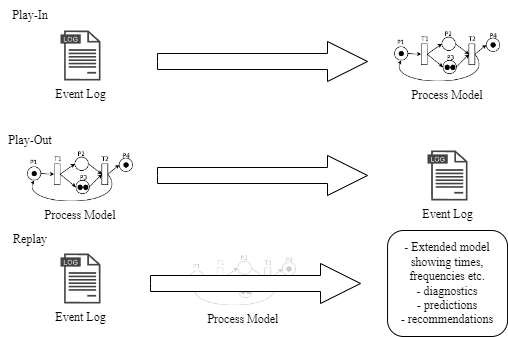
\includegraphics[width=0.8\textwidth]{figures/playinplayoutreplay.png}
  \caption{The Play-In, Play-Out and Replay concept in the context of process mining. The Play-In phase involves the creation of a process model from an event log. The Play-Out phase involves the creation of an event log from a process model. The Replay phase involves the modification of the process model thorough information gained from the event log.}
  \label{fig:playinoutreplay}
\end{figure}

Play-In refers to the creation of a process model out of an event log. Play-Out may be called "sampling" in data science as it generates traces out of the model. DES uses Play-Out to generate new exemplary behaviour, see \autoref{sec:material-flow}. Here, a process model may be used to play-out (simulate) several traces of the desired events and then use bagging techniques like averaging the durations per event to gain robust KPIs (\autoref{sec:relevant-kpis}) and to reduce variance. A biased process model may still generate biased KPIs. Replay uses event log and process model together to check conformance, enriching the model with information captured in the log or to transform a descriptive process model into a prescriptive one \autocite{van2016data}.

PM uses different formats to display process models like petri nets and BPMN models, among others \autocite{vanderAalst2012}. The thesis at hand focusses on DDDT in the context of simulation. Such data-driven models often come as a black box, thus they can not be rendered by PM models.

% Standards aus Will van der Aalst Buch beschreiben die hier einschlägig sind

\subsection{Object-Centricness in Process Mining}
\label{sec:object-centric-event-logs}

The problem with tranditional PM lies in its single dimensionality of perspective. For each process question, a new play-out has to be performed. Interactions between different objects are not captured \autocite{van2023object}. One event may be related to different cases (convergence) or from the perspective of a case, there may be several equal activities within a case (divergence) \autocite{van2019object}.
Recently, object-centric event data (OCED) have been proposed as a new data basis for PM \autocite{van2019object}. OCED logs (OCEL) are a generalization of classical event logs. Such traditional event logs use the case ID as a label to group and distringuish events. They assume that the process model describes the start and end of a single object. Each event refers to exactly one object (case) \autocite{van2023object}. OCED overthrows these assumptions by assuming that events may relate to multiple objects. To account for this new logic, OCEL coins the terms events, objects, types, attributes and qualifier. Each object has exactly one object type. Several objects may have the same type. An object type can be a description of the function such as machine, customer, supplier or activity descriptions such as invoice, request. Objects are instances of these types. Events in particular have an event type, termed activity. The same non-uniqueness applies here \textemdash many events can have the same type like "processing complaint", "cooking coffee". Each event is described by exactly one type. OCED assumes event atomicity; each event is indivisible. Each event has one timestamp. Compared to traditional PM, events may relate to multiple objects through a qualifier (E2O). Such a qualifier may be, considering the event "printing label" and object "printing station", the label to be printed. Objects may be related to multiple objects (O2O). O2O relationships are frozen (static) and are assumed to not change. The O2O relationship may be used to describe the order of producing a product. For example, the O2O relation "main pcb to gyroscope" may say that the main pcb has to be produced before the gyroscope. Another O2O relation can be an order, the connection between the customer object and the ordered product. It is worth mentioning that objects can also be related indirectly together through two E2O relations: The E2O relation "producing" may connect the event "machine 1 produces" with the object "gyroscope". The E2O relation "check" may connect the event "machine 1 checks" with the object "main pcb", thus connecting the two objects "gyroscope" and "main pcb" indirectly via two events \autocite{van2019object}. E2O relations are dynamic. They may change over time, involving different objects. In the given example, "main pcb" would be checked with "display" instead of "gyroscope".

Events and objects have attributes (keys), posessing values. Event attribute values refer to exactly one event and one event attribute, they are not shared. For example, the cost for one event may have the value $10€$. The same logic applies to objects as well, one event attribuite value refers to exactly one object and one object attribute. Because several events may have the same type and several objects may have the same type as well, each event- or object type may refer to any number of event or object attributes. They open interpretative possibilities for the modeller by considering them as expected attributes for the event or object type. The given example may be the event type "producing" which may have the event attribute "duration" and "cost". The object type "gyroscope" may have the object attribute "weight" and "size". One may averag the different object attribute values of one type cluster to generate object type KPIs. A key specificity of object attribute values lies in the fact that they have a timestamp. Event attribute values do not. Latter information would be redudant because events to already have a timestamp, see above. Event attribute values may have cardinality one per event. $N$ event attributes have $n$ values. This does not apply to object attribute values. They may have multiple values because of their nature to change over time \autocite{van2023object}. This is why each object attribute value has a timestamp. The attribute value is in conclusion unique for a given object during a given time given one attribute. The given example may be the object attribute "weight" of the object "main pcb" which may change over time. The object attribute value "weight" may have the value $100g$ at time $t_1$ and $120g$ at time $t_2$.

OCEL thus extends traditional PM by accommodating the  multi-object nature of complex processes. Unlike classical event logs—which restrict events to a single case—OCEL captures dynamic interactions among multiple objects via E2O relations and static inter-object dependencies through O2O relations. This enriched framework enables a more comprehensive representation of real-world processes, where events may concurrently affect several objects. Timestamped object attribution values enable the modeller to perform temporal analysis and KPI derivation (\autoref{sec:relevant-kpis}). Overall, OCED provides a more detailed, semantically rich representation of complex, interconnected processes. \autocite{van2023object}.

\subsection{Process Mining as Enabling Technology}
\label{sec:process-mining-enabling-technology}

Recall that PM uses event logs to develop process models or to enhance existing ones, so these logs may serve as a foundation for VVUQ of models in general. Live twin data often can be exported to the event log format. Several standardizations have been proposed, with the IEEE XES standard being the most widely used \autocite{van2016data}. The XES standard defines a common format for event logs, enabling the exchange of event data between different software frameworks. The idea lies in exporting twin decisions or live data as event logs and then use PM tools to perform VVUQ.
Replay may be used on SBDT simulated traces in comparison with actual event data to reveal mismatches in sequences or timing. For example, the SBDT could have predicted a circual process. Replay can be applied to further analyze this bottleneck. Play-Out can empower the modeller to sample a big amount of exemplary traces to gain KPIs. OCED object attribute values may offer even more insights.
PPC systems (\autoref{sec:ppc}) often times deliver even more data to enrich the event log so that VVUQ can be performed easier. If event log extraction out of the SBDT is performed online, VVUQ can be performed on the fly.

\section{VVUQ in the Context of Simulation-Based Digital Twins}
\label{sec:vvuq-sbdt}

The previous sections introduced the concepts of DES, PPC, relevant KPIs, DT, PM and OCED. This section now focusses on VVUQ in the context of SBDT. The thesis at hand uses the term VVUQ to describe the process of verifying, validating and quantifying the uncertainty of a SBDT. Verification and validation has a long history in manufacturing and DES \autocite{Bitencourt2023}. \Autocite{sel2025survey} add uncertainty quantification as a main interest. Their framework is applied in the medical domain, but they mention reasonable arguments regarding efficiency and safety of SBDT in general. Thus, the thesis considers VVUQ instead of merely verification and validation efforts. The following section introduces the basic concepts of VVUQ and its relevance for SBDT.


\subsection{Development process of VVUQ Concepts}
\label{sec:historical-development}
With the uprising of simulation models in the early 1950s \autocite{evans1967simulation}, the need for VVUQ arose unknowingly to the modellers. The usability of such simulations was deemed high as long as the results were promising, increasing trust in the technology \autocite{durst2017historical}. Blind trust does not validate models. Contrarily, if the results more or less were satisfactory, the model was considered validated \autocite{bonani2003physics}.

The first effort to define and perform verification was performed by \autocite{machlup1955problem} defining verification as "including the correctness of mathematical and logical arguments, the applicability of formulas and equations (...), the reliability and exactness of observations, the reproducability of experiments, the explanatory or predictive value of generalizations.". \Autocite{naylor1967verification} further refined this definitions by introducing the idea of "goodness of fit". Latter describes the capability of the model to correctly reflect the modelled system. During the 1970s, researchers like Schlesinger \autocite{schlesinger1979terminology} defined validation as achieving a "satisfactory range of accuracy consistent with the application", while Ignall argued for validation against simulations rather than analytical models \autocite{ignall1978using}. Sargent's work from 1979 to 1984 proposed methods like user collaboration and independent V&V, detailing techniques such as sensitivity analysis and Turing tests \autocite{Sargent2010wsc}. Balci developed a taxonomy and emphasized continuous V&V, reflecting the need for ongoing assessment \autocite{balci2012life}.

By 2004, modern V&V emerged. Considering model fidelity of today's approaches, \autocite{Oberkampf2004amr} introduced widely recognized definitions of V&V:

\begin{quote}
  \textit{Verification} is the process of determining that a model implementation accurately represents the developer's conceptual description of the model and the solution to the model.

  \textit{Validation} is the process of determining the degree to which a model is an accurate representation of the real world from the perspective of the intended uses of the model. \autocite{Oberkampf2004amr}
\end{quote}

Verification thus concerns itself with the correctness of the given model \autocite{Sargent2010wsc}, while validation evaluates the quality of explanations quantitavely \autocite{Oberkampf2004amr}. \Citeauthor{iso2017systems} span the concept of validation to computational models, where valid models correctly reflect the users intented functionality. PPC may provide the modeller with relevant KPIs to assess both.

\label{sec:uncertainty-quantification}
Uncertainty quantification (UQ) is a relatively new field in V&V. It aims to quantify the uncertainty of the model and its predictions through the whole lifecylce of the model, including training, inference and prediction \autocite{sel2025survey}. Uncertainty quantification empowers the modeller to define confidence intervals to correctly emphasize the stochastic nature of the model predictions \autocite{volodina2021importance}. This is crucial for SBDT, where real-time decisions rely on accurate representations, as \autocite{francis2021towards} highlights the need for continuous updates. UQ differentiates \textit{aleatory} uncertainty, which is inherent to the data, and \textit{epistemic} uncertainty, which is due to lack of knowledge \autocite{sel2025survey}. Aleatory uncertainty may arise due to sensor erros in the physical entity, generating noise. Epistemic uncertainty may arise due to lack of data or knowledge about the physical entity \autocite{thelen2023comprehensive}. Epistemic uncertainty can be reduced. \Autocite{abdoune2022handling} provide a comprehensive overview of UQ challenges and potential solutions in the context of SBDT.

For SBDT, VVUQ is not a one-time activity but a continuous process, ensuring digital twins mirror physical systems accurately. This is vital for industries like manufacturing, where decisions based on digital twins have significant implications \autoref{sec:problem}.
The historical development of VVUQ, from early verification to integrated UQ, reflects the growing complexity of simulation models. As SBDT become central to decision-making, robust VVUQ practices ensure reliability, linking back to foundational concepts introduced earlier, see \autoref{sec:types-digital-twins}. The concepts of VVUQ are embedded in the context of PM and OCED, which may further assist described endevours. Especially for UQ, PM offers a rich data source to quantify uncertainty and validate models by providing a \textit{degree of fit} of the given process model.


\subsection{VVUQ for Automatically Generated Models}
\label{sec:requirements-automatically-generated-models}
AMG stem largely stem from the DES discipline (\autoref{par:asmg:}), termed ASMG \autocite{mildeautomated,Charpentier2014}. They may use data-driven techniques which reduce the manual effort to create and update themselves. These models adapt quickly to changing conditions, making them valuable for dynamic environments like manufacturing. However, ensuring their reliability requires specific VVUQ. Because ASMG models often are black boxes, traditional VVUQ methods may not be applicable. The challenge lies in understanding the model's internal logic and ensuring it accurately reflects the physical system. If sophisticated data driven methods have been applied, several \textit{key challenges} arise, hindering successful VVUQ:

\begin{itemize}
  \item \textbf{Model Opacity:} ASMG models often use sophisticated machine learning algorithms like neural networks. Such black-box models are difficult to interpret, making it hard to understand their internal logic. This opacity may hinder VVUQ, as the modeller cannot easily identify errors or biases.
  \item \textbf{Data Dependency:} Data-driven models rely on high-quality data. If the data is biased or noisy, the model's predictions may be inaccurate.
  \item \textbf{Dynamic Model Adaptation:} Models that continuously learn and adapt, such as those employing online learning, require ongoing validation to ensure they remain valid as new data is ingested. This dynamic nature introduces the risk of concept drift \autocite{lu2018learning}, where the underlying process changes over time, potentially degrading model performance.
  \item \textbf{Quantifying Uncertainty:} Model predictions are stochastic in nature. For applications where precision is crucial, such as in manufacturing, uncertainty needs to be quantified.
\end{itemize}

To assess these challenges, the thesis defines the following \textit{key requirements} for VVUQ of automatically generated models, especially SBDT:
\begin{itemize}
  \item \textbf{Model Interpretability:} \label{par:surrogate} Ensuring the model's internal logic is transparent and understandable, enabling the modeller to identify errors or biases. Developing and employing techniques to make the decision-making processes of automatically generated models more transparent is crucial for VVUQ. Explainable AI methods, such as SHAP (SHapley Additive exPlanations, \autocite{lundberg2017unified}) or LIME (Local Interpretable Model-agnostic Explanations, \autocite{ribeiro2016should}), can help shedding light on model behavior, facilitating verification efforts. This is particularly important for black-box models like deep neural networks, where understanding the reasoning behind predictions is challenging. Often times, it may be easier to use white-box models like decision trees or linear regression models, which are interpretable by design. Such models are often times labeled transparent models. If black-box models are instead chosen, so called \textit{surrogate models} may be used to approximate the black-box model. The surrogate model is a white-box model, which is easier to interpret. This approach is called \textit{post-hoc} explanation \autocite{fischer2024demystifying}. SBDT generating explanations by themselves are the ultimate goal.
  \item \textbf{Upholding Data Quality:} Implementing procedures to ensure that the data used for model generation and validation is accurate, complete, and representative of the operational environment is vital. This includes data cleaning, preprocessing, and plausibility checks to identify and mitigate issues like missing values, outliers, or biases. For instance, in manufacturing digital twins, sensor data must be validated for accuracy and consistency to ensure reliable model outputs \autocite{rodriguez2023updating}.
  \item \textbf{Validatable Algorithms:} Besides ensuring model interpretability, the algorithms used for model generation must be validatable. Security risks are a huge concern for companies employing SBDT into their processes \autocite{alcaraz2022digital}. The algorithms used have to be secure, hardened against attacks. This is especially important for online learning algorithms, which may be vulnerable to adversarial attacks \autocite{balta2023digital}. Manipulated data may lead to incorrect model predictions, causing severe consequences in safety-critical applications like autonomous driving or medical diagnosis. Ensuring the robustness of the algorithms is crucial for reliable VVUQ.
  \item \textbf{Continuous Validation:} VVUQ processes have to work in real-time to ensure the model remains valid as new data is ingested. This requires continuous monitoring and validation of the model's predictions against real-world data. Techniques like online validation \autocite{francis2021towards} can help ensure the model's accuracy and reliability over time. This is particularly important for SBDT, which are designed to adapt to changing conditions and provide real-time insights. Continuous validation ensures the model remains reliable and trustworthy, even as the underlying process evolves.
  \item \textbf{Integration:} VVUQ processes have to be integrated into existing model- and PPC infrastructure to be able to perform VVUQ on the fly. This requires close collaboration between data scientists, domain experts, and IT specialists to ensure the seamless integration of VVUQ processes into the model lifecycle.
  \item \textbf{Scalability:} VVUQ processes have to be scalable as the underlying model or data evolves over time. This requires the development of scalable VVUQ techniques that can handle large volumes of data and complex models. Of course, the infrastructure must be able to handle the increased computational load.
\end{itemize}

As noted by \citeauthor{francis2021towards}, the lifecycle SBDT has implications for its VVUQ as well: VVUQ must accompany the SBDT in all phases, from conceptualization to deployment and operation. The key requirements outlined above provide a foundation for developing robust VVUQ processes for automatically generated models, ensuring their reliability and accuracy in real-world applications.

\subsection{Traditional versus Machine Learning-Based Approaches}
\label{sec:ml-approaches}

VVUQ can be performed using traditional methods or more sophisticated approaches. Traditional verification techniques may include code inspection, unit testing or debugging \autocite{maniaci2018verification}. If closed solutions to simulated models are available, they may be used to validate the simulation. Traditional validation techniques involve comparisons between model predictions and real-world data, such as statistical tests or sensitivity analysis. In the context of manufacturing, simple experiments or historical data can be used. The consultation of experts is another possibility \parencite{shao2023credibility}.

\subsubsection*{Machine Learning-Based VVUQ}

Sophisticated approaches may include the use of machine learning (ML) techniques to enhance VVUQ processes. ML can be used to identify patterns in data, detect anomalies, and improve model predictions. In addition to supervised and unsupervised learning shortly introduced in \autoref{sec:data-driven-digital-twins}, semi-supervised learning and reinforcement learning are two other approaches. Supervised learning may be employed where labels regarding the validity or non-validity of an OCEL (see \autoref{sec:object-centric-event-logs}) are given. Unsupervised learning may provide such labels as learned categories if they are missing or may assist with finding common patterns in the data. Unsupervised techniques are context-agnostic and assume no patterns in the data, see \citeauthor{hastie2009unsupervised} for the reverse problem of encoding a priori information in unsupervised algorithms. Semi-supervised learning combines labeled and unlabeled data to improve model performance. It somehow forms a middle ground where lots of unlabelled data is available and is then grouped by the algorithm. The scarce data is then used in the holdout set to perform testing \parencite{learning2006semi}. Reinforcement learning is not commonly applied in VVUQ of SBDT.
ML techniques are often referred to as "oracles" when used for VVUQ because of their key challenge of opacity \autoref{sec:requirements-automatically-generated-models}.

\subsubsection*{Challenges in Data Preparation and Feature Selection}

Before discussing the application of ML techniques in VVUQ, several problems hindering successful application of ML in VVUQ are identified. The first problem is data quality \parencite{wu2025uncertainty}. Data quality may degrade the performance and reliability of ML-based VVUQ approaches. Firstly, \textit{missing values} in the dataset can hinder the training process and potentially introduce biases. To account for this, imputation strategies or simply removing defect rows may be a solution \parencite{gudivada2017data}. The modeller has to keep in mind that this may corrupt the VVUQ process. Secondly \textit{outliers}, which are data points that deviate significantly from the rest, create a challenge as they might represent real trends in the data (and thus containing valuable edge cases for VVUQ) or simply be erroneous entries, requiring care of the modeller. Thirdly \textit{noise} can overblend the underlying patterns that ML algorithms aim to learn, reducing the accuracy and generalization ability of the VVUQ models \parencite{liu2020noise}. Such noise may be random, for example by measuring environmental influence, or systematic, for example emitted by erroneous sensors. The first kind of noise can be reduced by smooting or filtering.

Inconsistent data is another mistake to avoid in data gathering. It may arise from deviations in formats, units or representations of the same information. It can lead to confusion for ML algorithms and require standardization and cleaning \parencite{mahanthappa2021data}. Duplicate data entries may also generate false trends in the data. Imbalance introduced by duplicates or measurement erros can bias the model in predicting only the majority class when a classification problem is at hand.
Beyond data qualitiy, the modeller has to make sure that the data is representative and bias-free. The training data used for VVUQ models must accurately reflect the operational environment. Biases can arise through human intervention or environmental influence \parencite{liu2020noise}. Finally, the way data is split into training, testing, and validation sets is important for avoiding overfitting. Here, the model memorizes the training data and fails to generalize to unseen data.

After ensuring data quality, the modeller has to consider suitable features for the given problem. Features are columns in the dataset describing characteristics of the data points (rows) through values. OCEL provide a relatively strict feature set in which the modeller has to operate. This has the advantage that several of the upper challenges may be eliminated because the data can be exported through a standardized interface. Successful VVUQ methods may require additional features nontheless. Only the most relevant features may be selected \parencite{geron2022hands}. Feature engineering describes the endevour of creating new features through combining existing features or through a new data gathering process. The incorporation of features in model training is coined feature selection. In the given use case, an adaptive feature a feature selection based on twin components may be useful, see \autoref{sec:comparing-dmfs}.

\subsubsection*{Classification Methods for the Detection of Model Deviations}
\label{sec:classification-methods}
Extensive work has been done on the topic of ML-based deviation detection. Such deviations are called "anomalies" and the process is termed "anomaly detection" \parencite{kharitonov2022comparative}. Anomalies are data points that deviate significantly from the majority of the data. They can be classified into three categories: point anomalies, contextual anomalies and collective anomalies \parencite{chandola2009anomaly}. Point anomalies are single data points that differ significantly from the rest of the dataset. Contextual anomalies are data points that are normal in one context but anomalous in another. They appear less often than point anomalies and have less statistical weight. Collective anomalies are groups of data points that are anomalous when considered together but may not be anomalous individually. Anomalies are of special interest in the context of VVUQ, as they can indicate potential issues with the model or the data, see \autoref{sec:metrics}.

Several algorithms exist to detect anomalies, including statistical methods, clustering-based methods, and supervised learning methods. If the data is sufficiently labelled and preprocessed, supervised methods are promising. Algorithms such as Support Vector Machines (SVM), Neural Networks (NN), Decision Trees, and Random Forests can learn from this labeled data to classify new model outputs or behaviors as either normal or deviative. However, a common challenge in anomaly detection scenarios is the issue of class imbalance, where instances of normal behavior are more common than the occurrences of deviations. This imbalance needs to be carefully addressed during model training to prevent the classifier from being biased towards the majority class. Clustering-based unsupervised methods detect anomalies through grouping similar data points together. Algorithms like K-Means, DBSCAN, and Hierarchical Clustering can be used to identify clusters of normal behavior, with anomalies being those points that do not belong to any cluster. They measure the distance between data points to cull anomalous points as reaching far outside of a group of common data points. Often times the assigned groups can be plotted, yielding further insights in the nature of the detected anomalies. Statistical methods, on the other hand, rely on the assumption that the data follows a certain distribution. They identify anomalies based on statistical properties such as mean, variance, and standard deviation  \parencite{chandola2009anomaly}.

Anomaly detection and VVUQ share common goals of identifying deviations from expected behavior and ensuring the reliability of models. The two fields can benefit from each other, as VVUQ can provide a framework for evaluating the performance of anomaly detection algorithms, while anomaly detection techniques can enhance VVUQ processes by identifying potential issues in models or data.

\subsection{Modern VVUQ in the Context of SBDT}
\label{sec:vvuq-dt}
ML-based VVUQ approaches heavily rely on data. In the preceding sections, the thesis introduced several interfaces which may serve as suitable data sources. PM/OCED may provide event logs for VVUQ approaches \textemdash ML approaches can ingest those. PPC systems may provide additional data to enrich the event log. This section will shed light on a systematic literature review (SLR) on V&V in the context of DTs. After summarizing the main findings, several V&V approaches with increasing sophistication are presented. The section closes with a discussion of the most promising approaches.


\Autocite{Bitencourt2023} conducted a SLR on V&V in the context of DT \textemdash a relatively new field. They did not consider uncertainty quantification in their SLR. As \autocite{hua2022validation} note, there are no structured and established frameworks for validating DTs. This statement holds for all sectors where DTs are applied. The SLR analyzed 269 papers. They applied the 4R framework by \autocite{Osho2022jmsy} to describe the capabilities of the analyzed twin frameworks. The 4R framework consists of the four dimensions \textit{Representation}, \textit{Replication}, \textit{Reality} and \textit{No DT}. The SLR found that most frameworks ($49\%$) rather developed a DM or DS. Another $26\%$ of DT were only able to \textit{represent} the physical entity. Highly sophisticated DT were the exception, not the rule. Considering this trend, V&V may not be a topic researchers are interested in at first sight. \Autocite{Bitencourt2023} identified a trend throughout the years of increasing modelling capabilities of the considered DT. Up to the year 2023, the trend is still increasing. They identify more data sources as the main driver for this trend. From the 269 papers, $47\%$ have been applied in the manufacturing domain. Of all classified DT, one key insight is that most authors performed atleast one form of V&V.

\begin{figure}[htbp]
  \centering
  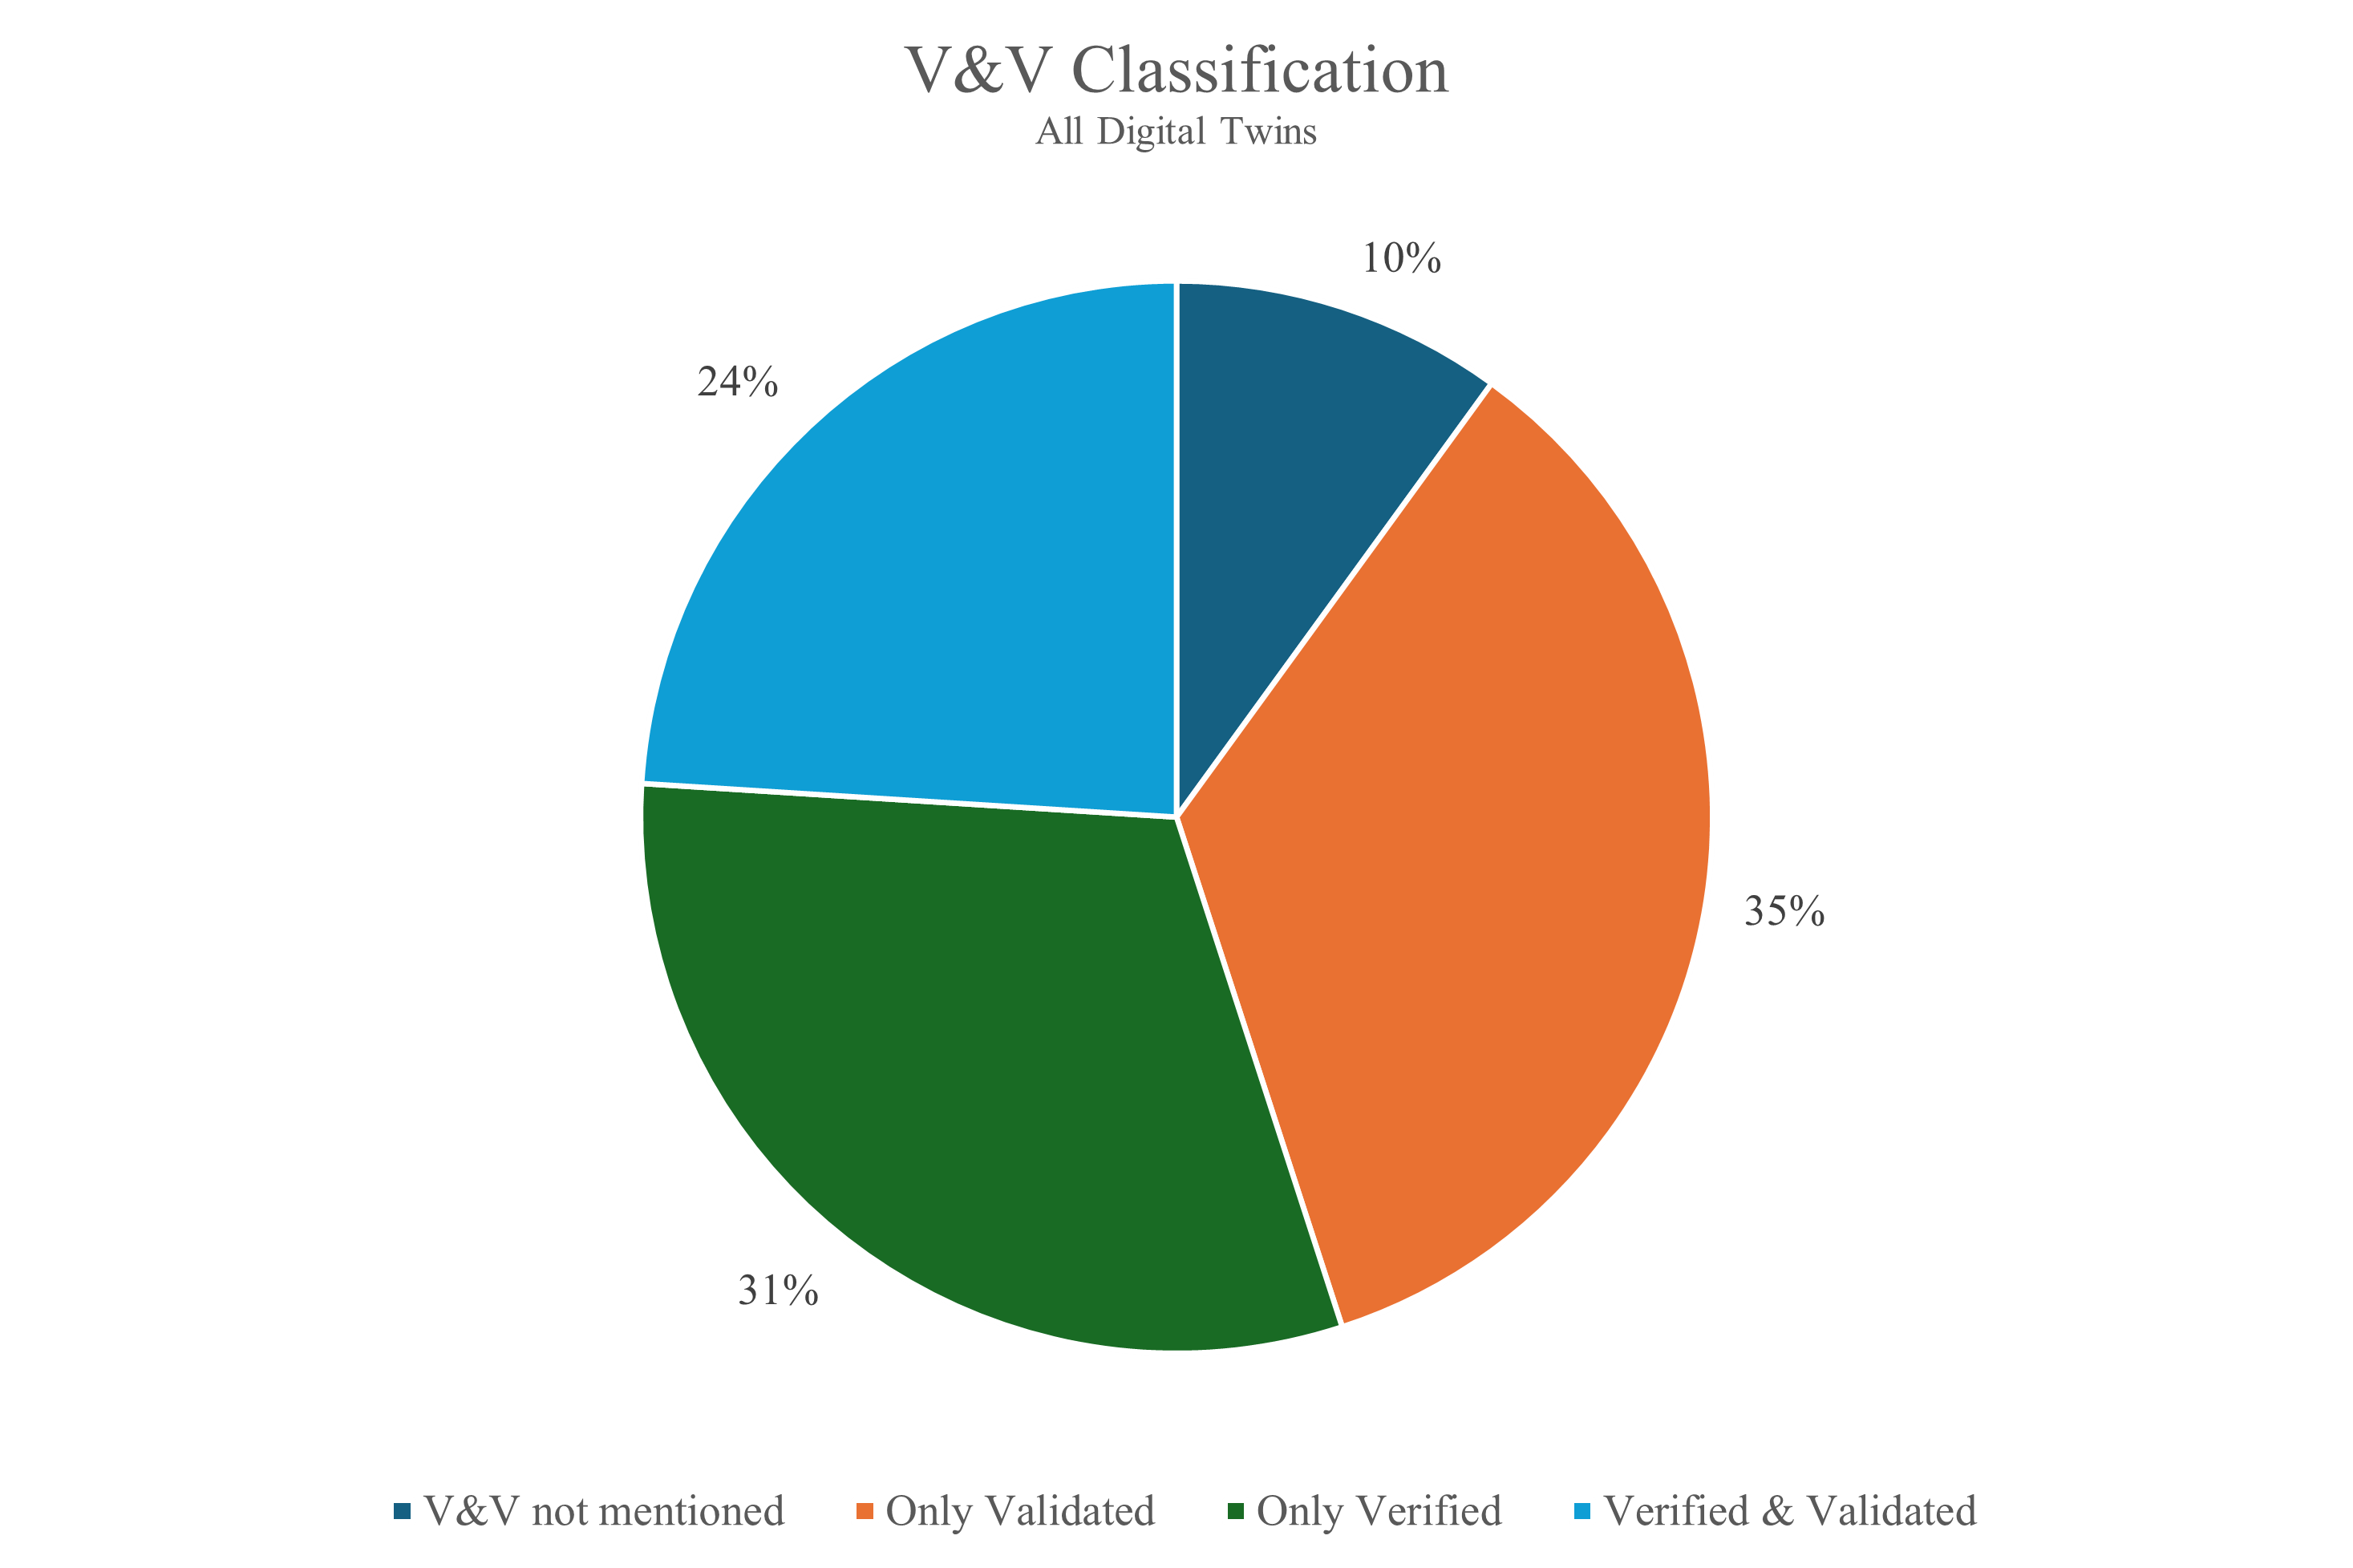
\includegraphics[width=0.8\textwidth]{figures/vvbitencourt.png}
  \caption{Donut chart showing the distribution of V&V methods in the context of DT.}
  \label{fig:vvbitencourt}
\end{figure}

DTs ranking in the \textit{reality} category where most often verified and validated. The authors deduct that because of the increasing complexity of the model, V&V may become a stressing topic. \Autocite{Nie2023rcim} propose a multi-agent and cloud-edge orchestration framework leveraging Digital Twin and IIoT to optimize distributed manufacturing resources. Their framework integrates a Convolutional Neural Network (CNN) with a bidirectional Long Short Term Memory (LSTM) module to perform scheduling and self-adaptive strategies for intelligent, real-time production control. They compare their network with an earlier adopted algorithm and its result to perform V&V. Quantifying the validity, they use Mean Squared Error (MSE) and Mean Absolute Error (MAE), see \autoref{sec:metrics}. This can still be considered manual VVUQ, because they did not use an automatic algorithm to compare the metrics of both models. PROOF
\Autocite{Lv2023rcim} defined target scenarios and boundaries to verify their DT for fault diagnosis of a drilling platform. They defined intervals for the metrics to be valid. Validation was performed by conducting a case study. Latter can be termed qualitative validation because the factual similarity of the case study against the DT has been assessed. Regarding their verification approach, they go one step further than \autocite{Nie2023rcim} by defining control intervals. This is somewhat automatic verification, but still requires human intervention when the values leave the defined intervals. \Autocite{Chen2023,Mykoniatis2021jim} both performed visual inspection to verify their DT. Both used cameras or other visual inspection tools to compare the DT results with reality. \Autocite{Chen2023} used thermal cameras to conduct temperature scans and compared the results with temperature prediction of the twin. \Autocite{Mykoniatis2021jim} used video recordings to validate their twin behaviour, but consulted KPIs to further validate their twin. Both approaches use aids for measurements and visual inspection. The measurements still have to be conducted and compared manually. Some authors performed statistical V&V, although the measurements were not automated. \Autocite{Wang2023asoc} compared historical data with the twin data and calculated the mean absolute percentage error of both datasets, \autoref{sec:metrics}. For validation they relied on conducting a case study, thus not fully automating V&V. \Autocite{Min2019ijinfomgt} performed verification using PPC KPIs, automating the V&V process even further. Their validation included using a validation set and measuring a set of metrics including error of fit and accuracy. This approach can be considered the first step towards a fully automated VVUQ process. \Autocite{Bitencourt2023} conclude that the majority of the analyzed papers performed V&V manually, with only a few authors automating the process. They also note that most authors did not consider uncertainty quantification in their work. And indeed, most work was performed in only conducting verification ($31\%$) where case studies were the method of choice \autocite{Eunike2022,jia2023from,kumbhar2023digital,Leng2020rcim,Leng2022aei}}. Case studies were also often applied where only validation tool place ($35\%$) \autocite{Alam2023,Dobaj2022,kherbache2022digital,Latsou2023,Leng2021jclepro,Negri2019promfg}. The SLR shows that V&V is a topic of interest in the context of DT, but most authors still rely on manual methods. The trend towards more sophisticated DTs and the increasing complexity of models will likely drive further research in this area. The SLR also highlights the need for more automated and standardized V&V processes, especially in the context of uncertainty quantification. Very few authors performed fully automated VVUQ for DT. The ones who did will now be discussed in more detail.


\subsubsection*{K-Nearest Neighbors (KNN) for Digital Twin Accreditation in Manufacturing}
The k-Nearest Neighbors (KNN) algorithm, a lazy learning approach grounded in measuring feature similarity, can be used for the accreditation of manufacturing digital twins \autocite{dos2024simulation}. KNN classifies new data points by identifying the majority class among the $K$ nearest neighbors in the training dataset. The determination of "being close" relies on various distance metrics. Most commonly, the Euclidean distance is used. Selecting an appropriate value for $K$ is crucial for balancing the model's bias and variance.
The approach by \autocite{dos2024simulation} integrates KNN with p-charts for the concurrent validation of SBDT \autocite{dos2024digital}. This involves monitoring the DTs output over time and using KNN to classify its behavior. Subsequently, p-charts are employed to statistically monitor the proportion of anomalies detected by KNN. The X-axis reprensents the discretized time $t$, the Y-axis represents the proportion of anomalies detected by the KNN. P-charts normally show a relative proportion of nonconforming items in a sample \autocite{acosta1999improved}. \Autocite{dos2024simulation} enriched their chart with an upper control limit (UCL) and lower control limit (LCL) which stand for acceptable statistical boundaries. This approach is similar to \autocite{Nie2023rcim} who also defined control intervals. If the p-value exceeds the boundaries, the twin may deviate from real behaviour. This method offers the advantage of real-time monitoring. However, it is sensitive to the choice of the hyperparameter $K$ and can be computationally expensive for large datasets \autocite{dos2024simulation}. The presence of outliers and noisy data can also impact the accuracy of KNN, and its performance may decrease in high-dimensional spaces. The authors utilized metrics such as accuracy, precision, recall and F1-Score (\autoref{sec:metrics}. They also used cross validation for increasing robustness of the prediction. By varying values for $K$, an optimal split may be found. Recalling the different kinds of anomalies from \autoref{sec:classification-methods}, KNN is able to capture point anomalies and contextual anomalies. Collective anomalies are not captured by KNN, as they are not able to learn from the data.

\subsubsection*{Time Series Classification for Fault Localization}
Time series classification techniques also play an important role in detecting and classifying anomalies within manufacturing digital twin systems \autocite{Lugaresi2023compind}. These techniques involve training classifiers on simulation data generated by the digital twin to identify and categorize faults in the real physical system \autocite{dihan2024digital}. A case study involving a scale-model gantry crane demonstrates the application of time series classification for this purpose \autocite{mertens2024localizing}.
Other techniques in this domain often involve deep learning models such as CNN, Recurrent Neural Networks (RNN), and LSTM networks. These models perform well at automatically extracting relevant features from time series data \autocite{cao2023real}, outperforming traditional rule-based or statistical methods in complex scenarios. Time series classification offers the benefits of automated anomaly detection and classification, with the potential for early fault prediction. However, a key challenge is the need for sufficient labeled data for training these models \autocite{zemskov2024security}, and real-time performance is often a critical requirement.

\subsubsection*{Uncertainty Quantification for Digital Twin Validation}
\label{sec:uq-dt}
V&V is an important aspect of SBDT, but uncertainty quantification (UQ) is equally crucial. UQ aims to quantify the uncertainty associated with the predictions made by the digital twin, providing insights into the reliability and confidence of its outputs \autocite{sel2025survey}. Certainity in predictions creates trust in the application, a desirable property of SBDT when used in practice \autocite{dwivedi2023explainable}. State of the art approaches to tackly uncertainty are Bayesian Neural Networks (BNN) \autocite{li2017dynamic}, Monte Carlo Dropout (MCD), Deep Ensembles (DE) and Gaussian Processes (GP). BNNs are able to quantify epistemic and aleatoric uncertainty (see \autoref{sec:uncertainty-quantification)}. They are a type of neural network that intoduce uncertainty into its predictions by treating the weights and biases as probability distributions rather than fixed values. Thus, each weight has a mean and a variance parameter for quantifying its uncertainty. During inference, samples are drawn from this distribution to \textit{learn} its characteristics. This allows the model to capture uncertainty in the data and make probabilistic predictions \autocite{li2017dynamic}. MCD, DE and GP train surrogate models (see \autoref{par:surrogate}) to approximate the uncertainty in the model's predictions.

MCD is a technique that uses dropout \autocite{srivastava2014dropout} during both training and inference phases to approximate the uncertainty in the model's predictions, unlike traditional dropout which is only used during training. By randomly dropping out neurons during inference with a chosen probability $p$, MCD generates multiple predictions, which then are averaged and can be used to estimate uncertainty. The key insight here is that effectively, the sampling happens from a dozen different NN because of their different weight configurations. We thus reach ensemble-learner like accuracy without the computational cost of training multiple complete models like in DE.
DE involves training multiple models with different initializations and architectures, and then combining their predictions to obtain a more robust estimate of uncertainty \autocite{rahaman2021uncertainty}. The difference between DE and MCD lies in statistically independent NNs, meaning they do not share statistical interaction processes. Furthermore, they are initialized randomly, whereas MCD networks share the same weight initialization. MCD and DE both provide good estimates for uncertainty, but it is recommended to apply both techniques after riguous fine-tuning of the DNN architechture \autocite{kamali2024advancements}.
GPs are a non-parametric Bayesian approach that models the underlying function as a distribution over functions \autocite{bilionis2012multi}. They provide a measure of uncertainty in their predictions by estimating the variance and mean of the predicted outputs \autocite{Burr2025TEADT}.

Overall VVUQ for SBDT is conducted with varying efforts. There is not a lot of research on fully automated VVUQ processes. The SLR by \autocite{Bitencourt2023} shows that most authors still rely on manual methods, if VVUQ has been performed at all. The trend towards more sophisticated DTs and the increasing complexity of models will likely drive further research in this area. The SLR also highlights the need for more automated and standardized VVUQ processes, especially in the context of uncertainty quantification. Very few authors performed fully automated VVUQ for DT. The ones who did were presented in this section.

\subsubsection*{Approaches not applied in VVUQ yet}
\label{sec:promising-future-directions}
This section closes with considering diverse promising approaches not yet applied in concurrent VVUQ of SBDT, which could address the limitations identified in existing methods.

The Local Outlier Factor (LOF) is a distance-based approach which identifies data points with high variance, thereby detecting outliers potentially connected to rare events or concept drift \autocite{alghushairy2020review}. Density-based methods, including Density-Based Spatial Clustering of Applications with Noise (DBSCAN), identify anomalies as data points placed in low-density regions \autocite{ccelik2011anomaly}. These methods can effectively distinguish between clusters of normal behavior and deviations that fall outside these typical regions.
The Isolation Forest algorithm offers an efficient approach for high-dimensional data by isolating anomalies through random data partitioning, where anomalies, being rare by nature, tend to be isolated more quickly than normal data points \autocite{xu2017improved}.
One-Class Support Vector Machines (OCSVM) learn a boundary that capture the normal data, identifying any instances falling outside this region as anomalies \autocite{li2003improving}. This method is especially useful when only data representing normal SBDT behavior is readily available, allowing the model to learn the manifold of "normal" operations and flag any future deviations. NN-based methods, particularly autoencoders (AE) \autocite{zhou2017anomaly}, can be trained on normal SBDT data to learn a compressed representation and then reconstruct the original data. Anomalies typically exhibit higher errors when the AE tries to reconstruct the default behaviour, making them detectable. These methods are capable of learning complex, non-linear patterns in SBDT behavior and are effectively identify subtle deviations. Furthermore, semi-supervised techniques can enhance deviation detection by leveraging a small amount of labeled anomaly data in comparison with a larger set of normal data. \(\blacksquare\)

This chapter established the theoretical foundation for the research presented in this thesis. It began by introducing DMFS and their simulation using DES, differentiating static and dynamic components. The discussion highlighted the connection between PPC and data quality. KPIs were identified as critical tools for balancing the inherent trade-offs between model accuracy, computational efficiency, and scalability \textemdash an omnipresent challenge in SBDT \autoref{sec:problem}.

The chapter then explored the concept of DT, SBDT, DDDT, and HDT. Each type was analyzed for its strengths and limitations, with SBDT relying on DES for dynamic representation, DDDT using machine learning for automated adaptation, and HDT combining domain knowledge with data-driven insights. PM was mentioned as a useful tool for DT validation, particularly through object-centric event logs (OCEL), which provide a multi-dimensional perspective on process interactions. OCEL’s ability to capture complex, concurrent relationships between objects and events positions it as a powerful tool for enhancing traditional PM techniques.

Finally, the chapter addressed VVUQ as essential processes for ensuring the reliability of SBDT. Traditional VVUQ methods, such as statistical tests were compared with modern machine learning approaches, including KNN and BNN. This highlights the need for continuous, automated VVUQ frameworks capable of handling the dynamic nature of SBDT. Key challenges such as model opacity, data dependency, and uncertainty quantification were identified as critical areas for future research. Key requirements for successful VVUQ were developed.

These theoretical components \textemdash DMFS modeling, DT architectures, PM/OCEL integration, and advanced VVUQ techniques \textemdash form the foundation for this thesis. The next chapter will present the methodology employed to develop a framework for VVUQ of SBDT, addressing the challenges and opportunities identified in this chapter. The goal of the framework is to enhance the reliability and accuracy of SBDT in real-world applications.




